\section{Auswertung}
\label{sec:Auswertung}
Alle in der Auswertung benutzten Mittelwerte werden über die Gleichung
\begin{equation}
\tilde{x}=\frac{1}{n}\sum_{i=1}^n {x_i}
\end{equation}
bestimmt. Die Standardabweichung der Mittelwerte ergibt sich zu 
\begin{equation}
\Delta{\tilde{x}}=\sqrt{\frac{1}{n(n-1)}\sum_{i=1}^n {(x_i-\tilde{x})²}}.
\end{equation}
Wird eine Größe bestimmt, welche sich aus fehlerbehafteten Daten zusammensetzt, ergibt sich der absolute Fehler über die \textsc{Gauss}schen Fehlerfortpflanzung 
\begin{equation}
\Delta{f}(x_1,..,x_n)=\sqrt{\left(\frac{\mathup{d}f}{\mathup{d}x_1}\Delta{x_1}\right)²+..+\left(\frac{\mathup{d}f}{\mathup{d}x_n}\Delta{x_n}\right)²}.
\end{equation}
Zur Berechnung aller Größen werden die nicht gerundeten Größen benutzt um Rundungsfehler zu vermeiden. Am Ende der Auswertung aller Größen werden diese auf die erste signifikante Stelle des Fehlers gerundet. 

In den gemessenen Zeiten $t_\mathup{auf}$, $t_\mathup{ab}$ und $t_0$ überwinden die Öltropfen eine Strecke von $s=\SI{0.5}{\milli\meter}$.
Aufgetragen sind die Messwerte in den Tabellen \ref{tab:T1} bis \ref{tab:T5}. Die Temperatur innerhalb der Ölkammer ändert sich im Laufe des Versuches nur sehr geringfügig.
\begin{table}[p]
\begin{minipage}[t]{0.5\linewidth}
	\begin{center}
	\sisetup{table-format=2.2}
	\begin{tabular}{S[table-format=1.0] S S}
		\toprule
		{Tröpfchen} & {$t_\mathup{auf}\:/\si\second$} &{$t_\mathup{ab}\:/\si\second$} \\
		\midrule
1 & 46.72 & 13.76\\
  & 45.20 & 15.41\\
  & 42.66 & 13.66\\
2 &  4.32 &  3.52\\
  &  8.60 &  7.09\\
  &  8.78 &  4.06\\
3 &  6.83 &  5.16\\
  &  7.15 &  5.56\\
  &  7.00 &  5.69\\
4 & 12.53 &  7.95\\
  & 13.75 &  7.53\\
  & 12.16 &  7.29\\
5 & 31.50 & 13.83\\
  & 28.87 & 11.64\\
  & 22.32 & 10.89\\
		\bottomrule
	\end{tabular}
	\caption{$U=\SI{200}{\volt}$,\,$T=\SI{300.15}{\kelvin}$.} 
	\label{tab:T1}
\end{center}
 \end{minipage}
    \hfill
    \begin{minipage}[t]{0.5\linewidth}
\begin{center}
	\sisetup{table-format=2.2}
	\begin{tabular}{S[table-format=1.0] S S}
		\toprule
		{Tröpfchen} & {$t_\mathup{auf}\:/\si\second$} &{$t_\mathup{ab}\:/\si\second$} \\
		\midrule
 6 & 12.18 & 8.26 \\
   & 13.84 & 9.01\\
   & 12.43 & 8.63\\
 7 &  9.69 & 6.16\\
   &  7.29 & 6.41\\
   &  7.72 & 6.73\\
 8 &  9.09 & 7.56\\
   &  9.32 & 8.26\\
   &  9.20 & 8.23\\
 9 &  8.76 & 6.36\\
   &  9.09 & 5.52\\
   &  8.33 & 6.00\\
10 & 11.81 & 9.29\\
   & 12.03 & 7.00\\
   & 11.72 & 8.75\\
		\bottomrule
	\end{tabular}
	\caption{$U=\SI{225}{\volt}$,\,$T=\SI{301.15}{\kelvin}$.} 
	\label{tab:T2}
\end{center}
\end{minipage}
\end{table}

\begin{table}[p]
\begin{minipage}[t]{0.5\linewidth}
	\centering
	\sisetup{table-format=2.2}
	\begin{tabular}{S[table-format=1.0] S S}
		\toprule
		{Tröpfchen} & {$t_\mathup{auf}\:/\si\second$} &{$t_\mathup{ab}\:/\si\second$} \\
		\midrule
11 &  9.36 &  9.07\\
   &  9.66 &  6.20\\
   &  9.52 &  7.20\\
12 & 12.52 &  9.26\\
   & 11.84 &  9.10\\
   & 12.13 &  9.30\\
13 &  6.06 &  5.64\\
   &  7.28 &  5.60\\
   &  6.90 &  5.83\\
14 & 36.47 & 12.03\\
   & 36.76 & 14.33\\
   & 36.60 & 16.72\\
15 & 12.96 &  9.03\\
   & 13.32 &  7.32\\
   & 14.61 &  8.91\\
		\bottomrule
	\end{tabular}
	\caption{$U=\SI{250}{\volt}$,\,$T=\SI{301.15}{\kelvin}$.} 
	\label{tab:T3}
\end{minipage}
\hfill
    \begin{minipage}[t]{0.5\linewidth}
	\centering
	\sisetup{table-format=2.2}
	\begin{tabular}{S[table-format=1.0] S S}
		\toprule
		{Tröpfchen} & {$t_\mathup{auf}\:/\si\second$} &{$t_\mathup{ab}\:/\si\second$} \\
		\midrule
16 & 12.30 & 11.10 \\
   & 14.90 & 10.86 \\
   & 13.49 & 10.33 \\
17 &  8.30 &  5.90 \\
   &  8.41 &  6.12\\
   &  8.58 &  5.96 \\
18 & 12.35 &  7.30 \\
   & 11.76 &  6.87 \\
   & 12.00 &  9.63 \\
19 & 17.62 & 13.66\\
   & 13.18 & 10.66\\
   & 16.84 & 13.07\\
20 &  1.90 &  1.60 \\
   &  2.10 &  1.55 \\
   &  2.24 &  2.07 \\
		\bottomrule
	\end{tabular}
	\caption{$U=\SI{275}{\volt}$,\,$T=\SI{301.15}{\kelvin}$.} 
	\label{tab:T4}
\end{minipage}
\end{table}


\begin{table}[p]
	\centering
	\sisetup{table-format=2.2}
	\begin{tabular}{S[table-format=1.0] S S}
		\toprule
		{Tröpfchen} & {$t_\mathup{auf}\:/\si\second$} &{$t_\mathup{ab}\:/\si\second$} \\
		\midrule
21 &  7.00 & 6.03\\
   &  7.14 & 6.31\\ 
   &  7.45 & 5.89\\
22 &  9.66 & 4.09\\
   &  8.26 & 4.46\\
   &  8.73 & 4.14\\
23 &  4.30 & 3.83\\
   &  4.45 & 4.75\\
   &  4.56 & 4.33\\
24 & 10.73 & 4.98\\
   &  6.51 & 6.31\\
   &  7.15 & 5.03\\
25 &  9.25 & 5.01\\
   &  8.36 & 3.97\\
   &  8.78 & 4.14\\
		\bottomrule
	\end{tabular}
	\caption{$U=\SI{300}{\volt}$,\,$T=\SI{301.15}{\kelvin}$.} 
	\label{tab:T5}
\end{table}

In Tabelle \ref{tab:werte} sind die berechneten Fallgeschwindigkeiten und deren Fehler aufgelistet.
Es gehen nur die Tröpfchen in die folgende Auswertung ein, welche die Gleichung 
\begin{equation}
2v_0\approx v_\mathup{ab}-v_\mathup{auf}
\label{eq:plaus_test}
\end{equation}
 erfüllen. 
Ist dies nicht der Fall, so haben die Tröpfchen während der Messung ihre Ladung geändert.
 Dadurch sind sie zur Bestimmung der Elementarladung $e$ unbrauchbar.
\begin{table}
	\centering
	\sisetup{table-format=2.2}
	\begin{tabular}{S[table-format=2.0] S[table-format=3.0] S[table-format=1.6] S[table-format=1.6] S[table-format=1.4] S[table-format=1.4]S[table-format=1.3]}
		\toprule
		{Tröpfchen}& {$U\:/\si{\volt}$} & {$v_\mathup{auf}\:/\frac{\si{\milli\meter}}{\si\second}$} &{$\Delta{v}_\mathup{auf}\:/\frac{\si{\milli\meter}}{\si\second}$} & {$v_\mathup{ab}\:/\frac{\si{\milli\meter}}{\si\second}$} &{$\Delta{v}_\mathup{ab}\:/\frac{\si{\milli\meter}}{\si\second}$}&{$v_0\:/\frac{\si{\milli\meter}}{\si\second}$} \\
		\midrule
 1  & 200   &   0.0111    & 0.0003     & 0.035     & 0.001     & 0.013   \\
 2  & 200   &   0.07      & 0.02       & 0.11      & 0.02      & 0.009   \\
 3  & 200   &   0.0715    & 0.001      & 0.091     & 0.003     & 0.009   \\ 
 4  & 200   &   0.039     & 0.001      & 0.065     & 0.002     & 0.014   \\
 5  & 200   &   0.018     & 0.002      & 0.041     & 0.003     & 0.010   \\
 6  & 225   &   0.0394    & 0.002      & 0.057     & 0.001     & 0.008   \\
 7  & 225   &   0.061     & 0.005      & 0.077     & 0.002     & 0.009   \\
 8  & 225   &   0.0543    & 0.0004     & 0.062     & 0.002     & 0.007   \\
 9  & 225   &   0.0573    & 0.001      & 0.084     & 0.003     & 0.008   \\
10  & 225   &   0.0421    & 0.0003     & 0.060     & 0.005     & 0.008   \\
11  & 250   &   0.0525    & 0.0005     & 0.068     & 0.007     & 0.008   \\
12  & 250   &   0.0411    & 0.0007     & 0.0542    & 0.0004    & 0.008   \\
13  & 250   &   0.074     & 0.004      & 0.087     & 0.001     & 0.010   \\
14  & 250   &   0.013655  & 0.00003    & 0.035     & 0.003     & 0.010   \\
15  & 250   &   0.036     & 0.001      & 0.059     & 0.004     & 0.008   \\
16  & 275   &   0.037     & 0.002      & 0.046     & 0.001     & 0.010   \\
17  & 275   &   0.0593    & 0.0006     & 0.0834    & 0.0009    & 0.023   \\
18  & 275   &   0.0415    & 0.0006     & 0.064     & 0.006     & 0.010   \\
19  & 275   &   0.032     & 0.003      & 0.040     & 0.003     & 0.008   \\
20  & 275   &   0.24      & 0.01       & 0.29      & 0.03      & 0.014   \\
21  & 300   &   0.069     & 0.001      & 0.082     & 0.002     & 0.010   \\
22  & 300   &   0.056     & 0.003      & 0.118     & 0.003     & 0.012   \\
23  & 300   &   0.112     & 0.002      & 0.117     & 0.007     & 0.011   \\
24  & 300   &   0.064     & 0.009      & 0.093     & 0.007     & 0.009   \\
25  & 300   &   0.056     & 0.002      & 0.115     & 0.008     & 0.010   \\
		\bottomrule
	\end{tabular}
	\caption{} 
	\label{tab:werte}
\end{table}

Nach \eqref{eq:radius} und \eqref{eq:ladung} werden Radien $r$ und Ladungen $q$ der Tröpfchen mit absolutem Fehler bestimmt.
Gemäß der Geradengleichung
\begin{equation}
\eta_\mathup{Luft}=47,0580\cdot10⁻¹⁹\,\frac{\si{\newton\second}}{\si{\kelvin{\meter}²}\cdot T + 4,4433\cdot10⁻⁶\,\frac{\si{\newton\second}}{\si{{\meter}²}}}
\end{equation}
wird $\eta_\mathup{Luft}$ ermittelt. Der lineare Zusammenhang zwischen Temperatur und Viskosität ist dargestellt in Abbildung \ref{fig:temp}.
\begin{landscape}
    \begin{table}
        \begin{center}
            \begin{tabular}{c S[table-format=1.4] S[table-format=1.1] S[table-format=1.2] S[table-format=1.3] S[table-format=1.2] S[table-format=3.1]}
		\toprule
		{Tröpfchen} & {$\eta\:/10⁻⁵\frac{\si{\newton\second}}{{\si\meter²}}$} &{$r\pm\Delta{r}\:/10⁻⁷\si\meter$}&{$q\pm\Delta{q}\:/10⁻¹⁹\si\coulomb$}&{$\eta_C\pm\Delta{\eta_C}\:/10⁻⁵\frac{\si{\newton\second}}{{\si\meter²}}$}&{$q_C\pm\Delta{q_C}\:/10⁻¹⁹\si\coulomb$}&{$\Delta_{rel}{q_C}\:/\%$} \\
		\midrule
 1  & 1.8568  & 4.8 $\pm$ 0,1  & 1.0  $\pm$ 0,1  & 1.584  $\pm$ 0,007 &  1.3 $\pm$   0,2  &   15.4\\
 2  & 1.8568  & 6   $\pm$ 2    & 5    $\pm$ 5    & 1.63   $\pm$ 0,08  &  6   $\pm$   6    &  100.0\\
 3  & 1.8568  & 4.4 $\pm$ 0,3  & 3.4  $\pm$ 0,6  & 1.56   $\pm$ 0,02  &  4.4 $\pm$   0,8  &   18.2\\
 4  & 1.8568  & 5.1 $\pm$ 0,2  & 2.5  $\pm$ 0,2  & 1.597  $\pm$ 0,009 &  3.2 $\pm$   0,3  &    9.4\\
 5  & 1.8568  & 4.7 $\pm$ 0,4  & 1.3  $\pm$ 0,3  & 1.58   $\pm$ 0,02  &  1.7 $\pm$   0,4  &   23.5\\
 6  & 1.8615  & 4.3 $\pm$ 0,2  & 1.7  $\pm$ 0,2  & 1.56   $\pm$ 0,01  &  2.3 $\pm$   0,3  &   13.0\\
 7  & 1.8615  & 3.9 $\pm$ 0,7  & 2.3  $\pm$ 0,7  & 1.54   $\pm$ 0,05  &  3.1 $\pm$   0,9  &   29.0\\
 8  & 1.8615  & 2.8 $\pm$ 0,3  & 1.4  $\pm$ 0,4  & 1.44   $\pm$ 0,04  &  2.0 $\pm$   0,5  &   25.0\\
 9  & 1.8615  & 5.1 $\pm$ 0,4  & 3.0  $\pm$ 0,6  & 1.69   $\pm$ 0,02  &  3.8 $\pm$   0,7  &   18.4\\
10  & 1.8615  & 4.2 $\pm$ 0,6  & 1.8  $\pm$ 0,7  & 1.56   $\pm$ 0,04  &  2   $\pm$   1    &   50.0\\
11  & 1.8615  & 3.9 $\pm$ 0,9  & 2    $\pm$ 1    & 1.54   $\pm$ 0,06  &  2   $\pm$   1    &   50.0\\
12  & 1.8615  & 3.6 $\pm$ 0,1  & 1.28 $\pm$ 0,07 & 1.510  $\pm$ 0,008 &  1.76$\pm$   0,09 &    5.1\\
13  & 1.8615  & 3.6 $\pm$ 0,6  & 2.2  $\pm$ 0,6  & 1.51   $\pm$ 0,05  &  3.0 $\pm$   0,8  &   26.7\\
14  & 1.8615  & 4.6 $\pm$ 0,4  & 0.9  $\pm$ 0,2  & 1.58   $\pm$ 0,02  &  1.1 $\pm$   0,3  &   27.3\\
15  & 1.8615  & 4.7 $\pm$ 0,4  & 1.7  $\pm$ 0,5  & 1.58   $\pm$ 0,02  &  2.2 $\pm$   0,6  &   27.8\\
16  & 1.8615  & 3.0 $\pm$ 0,4  & 0.9  $\pm$ 0,2  & 1.46   $\pm$ 0,04  &  1.2 $\pm$   0,3  &   25.0\\
17  & 1.8615  & 4.8 $\pm$ 0,1  & 2.4  $\pm$ 0,1  & 1.589  $\pm$ 0,005 &  3.0 $\pm$   0,2  &    6.7\\
18  & 1.8615  & 4.7 $\pm$ 0,7  & 1.7  $\pm$ 0,7  & 1.58   $\pm$ 0,03  &  2.2 $\pm$   0,9  &   40.9\\
19  & 1.8615  & 2.9 $\pm$ 0,7  & 0.7  $\pm$ 0,4  & 1.45   $\pm$ 0,08  &  1.0 $\pm$   0,6  &   60.0\\
20  & 1.8615  & 7   $\pm$ 2    & 12   $\pm$ 8    & 1.66   $\pm$ 0,05  & 15   $\pm$ 10     &   66.7\\
21  & 1.8615  & 3.5 $\pm$ 0,3  & 1.7  $\pm$ 0,3  & 1.51   $\pm$ 0,02  &  2.3 $\pm$   0,4  &   17.4\\
22  & 1.8615  & 7.7 $\pm$ 0,3  & 4.3  $\pm$ 0,4  & 1.682  $\pm$ 0,005 &  5.0 $\pm$   0,4  &    8.0\\
23  & 1.8615  & 2.0 $\pm$ 2,0  & 1    $\pm$ 3    & 1.3    $\pm$ 0,3   &  2   $\pm$   5    &  250.0\\
24  & 1.8615  & 5   $\pm$ 1    & 3    $\pm$ 1    & 1.61   $\pm$ 0,04  &  3   $\pm$   1    &   33.3\\
25  & 1.8615  & 7.5 $\pm$ 0,5  & 4.1  $\pm$ 0,9  & 1.68   $\pm$ 0,01  &  5   $\pm$   1    &   20.0\\
		\bottomrule
           \bottomrule
            \end{tabular}
        \end{center}
\caption{Ergebnisse der Berechnung zur Bestimmung der Ladung eines Öltröpfchens.}
        \label{tab:ergebnisse}
    \end{table}
\end{landscape}

%%%%%%%%%%%%%%%%%%%%%%%Das noch in die Theorie mit einbauen%%%%%%%%%%%%%%%%%
%Durch das Zerstäuben der Öltröpchen ist deren Durchmesser so gering, dass er sich in ähnlichen Größenordnungen bewegt wie die mittlere freie Weglänge der Moleküle, welche sich in der Luft befinden. Die Stokesche Reibung wird hier ungenau und muss durch eine Korrektur behoben werden. Diese wurde 1910 vom Mathematiker Ebenezer Cunningham abgeleitet.
Die \textsc{Cunningham}-Korrektur der Viskosität nach Gleichung \eqref{eq:cunningham} fließt in die Berechnung der Ladung mit ein, deswegen wird erneut die Ladung $q_\mathup{C}$ und Fehler dieser mit Korrekturfaktor bestimmt.
Messbedingt treten teilweise sehr große Fehler auf, wie in Tabelle \ref{tab:ergebnisse} zu sehen ist. Deswegen werden alle Werte mit einem relativen Fehler größer als $20\%$ aus der Rechnung herausgenommen.
\begin{figure}
	\centering
	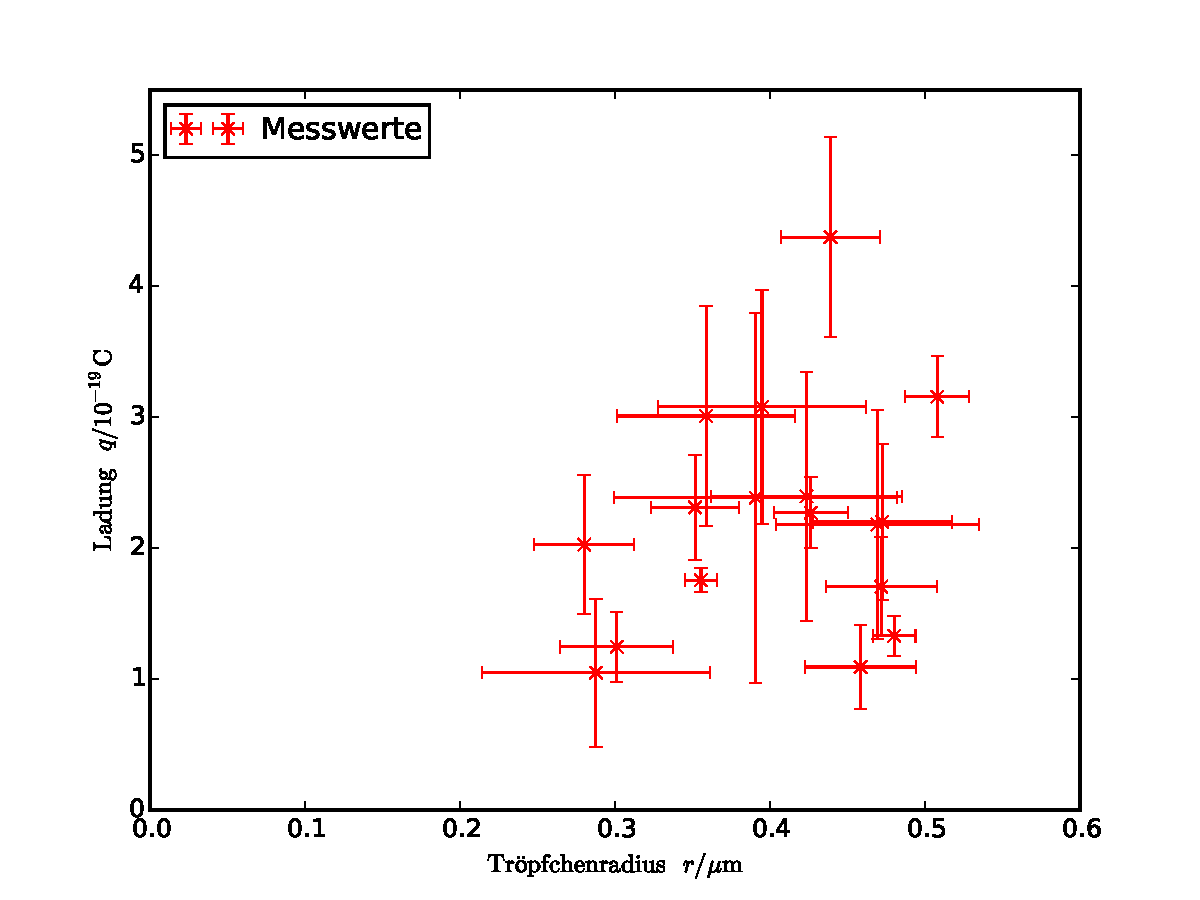
\includegraphics[width=\textwidth]{Bilder/plot_messwerte.pdf}
	\caption{Ladungen $q$ der Tröpfchen aufgetragen gegen den Radius $r$.}
	\label{fig:1}
\end{figure}
Nun wird die berechnete Ladung der Tröpfchen in Abbildung \ref{fig:1} gegen ihren Radius aufgetragen. Tropfen mit größerem Radius tragen prinzipiell mehr Ladung als Tröpfchen mit kleinem. Untersucht werden hauptsächlich Tröpfchen mit geringem Radius und wenig Ladung, welches eine langsamere Geschwindigkeit hevorruft.
Gemäß der Annahme, dass Ladung quantisiert ist, müssen die Öltropfen immer genau die Elementarladung oder ein Vielfaches derer tragen. Zur Bestimmung der Elementarladung muss der größte gemeinsame Teiler der berechneten Ladungen gefunden werden. Da die Größen fehlerbehaftet sind wird ein Algorithmus zur Auswertung herangezogen.
Der gesuchte Wert für $e$ wird vom Computer zu $e'$ "erraten", falls ein in frage kommender eingegrenzter Bereich vorgegeben wird. Dies setzt voraus, dass die ungefähre Größenordnung der Elementarladung bekannt ist. Ausgewählt wird der Bereich zwischen $1,0\cdot 10⁻¹⁹\,\si\coulomb$ und $1,8\cdot 10⁻¹⁹\,\si\coulomb$. Es wird berechnet, um welchen Wert die gemessenen Ladungen von der "geratenen" Ladung bzw. deren Vielfachen abweichen. Die Abweichungen aller nach \textsc{Cunningham} korregierten Ladungen $q_C$ werden aufsummiert. Anschließend wird der Mittelwert gebildet. Daraus kann für jede geratene Ladung eine mittlere Abweichung der Messwerte bestimmt werden. Ist diese Abweichung minimal ist die Elementarladung gefunden. Die mittlere relative Abweichung des Ladungsvielfachen von der geratenen Ladung ist

\begin{equation}
\tilde{\Delta{q}}=\frac{1}{N}\sum i=1_N \left(1-\frac{q_i\left(\frac{q_i}{e'}\right)⁻¹}{e'}\right).
\end{equation}
\begin{figure}
	\centering
	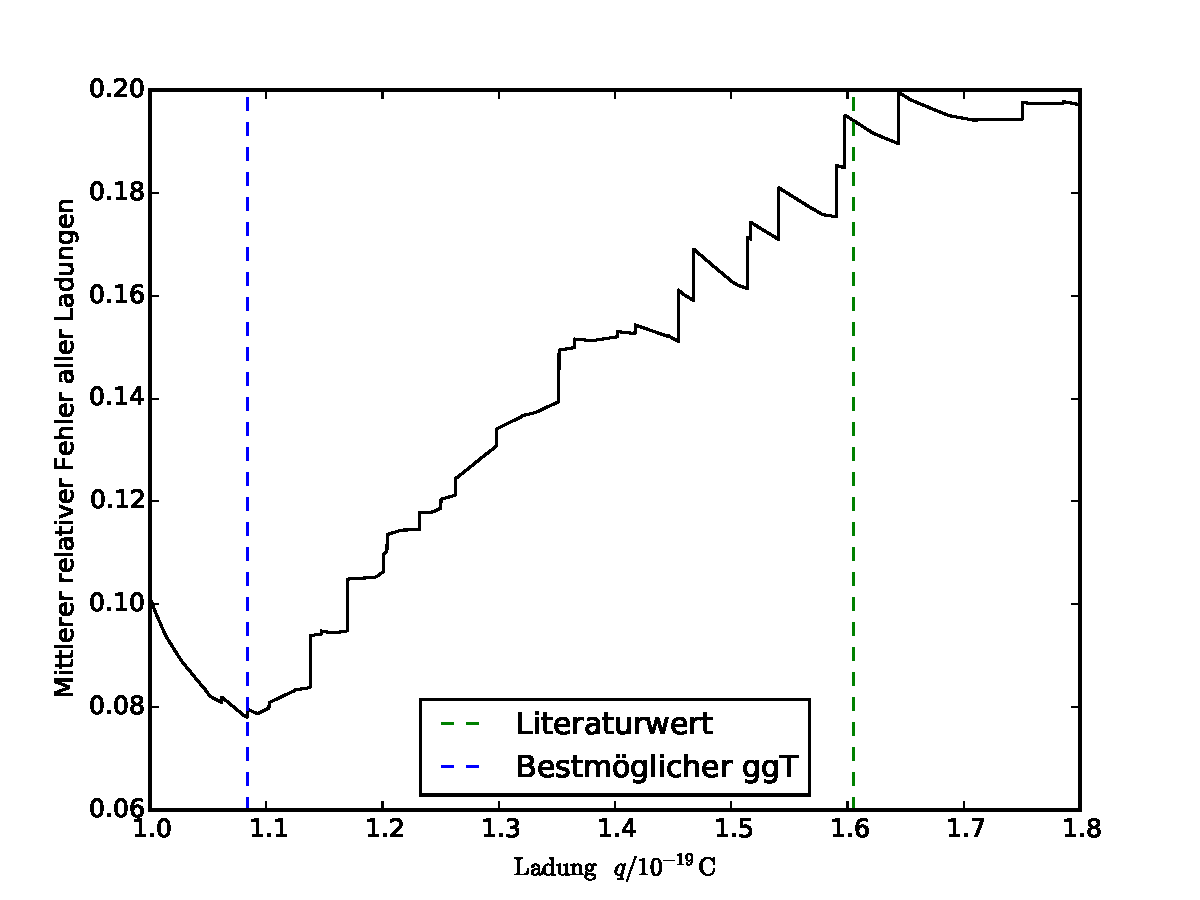
\includegraphics[width=\textwidth]{Bilder/plot_ggT}
	\caption{Bestimmung des größten gemeinsamen Teilers.}
	\label{fig:2}
\end{figure}
In Abbildung \ref{fig:2} wird der mittlere relative Fehler aller Ladungen gegen diese aufgetragen. Der kleinste gemeinsame Teiler bei $e=1,084\cdot10⁻¹⁹\,\si\coulomb$ entspricht der Elementarladung. Diese weicht stark vom ebenfalls eingezeichneten Literaturwert \cite{texas_instruments1} ab. 

\subsection{Bestimmung der \textsc{Avogadro}-Konstante}

Die \textsc{Avogadro}-Konstante wird bestimmt über die vorherig berechnete Elementarladung $e$ und die als gegeben vorausgesetzte \textsc{Faraday}-Konstante. Sie beschreibt nach Gleichung \eqref{eq:av} die Ladung eines Mols einfach geladener Ionen. Wird $F$ durch die Ladung geteilt ergibt sich die Anzahl der Teilchen in einem Mol zu $N_\mathup{A}=\frac{F}{e_0}=8,905\cdot10²³\frac{1}{\si\mol}$. Dieser Wert weicht, bedingt durch die starke Abweichung der Elementarladung, relativ stark vom Literaturwert \cite{texas_instruments3} mit $\tilde{N}_\mathup{A}=6,022\cdot10²³\frac{1}{\si\mol}$ ab.
\begin{figure}
	\centering
	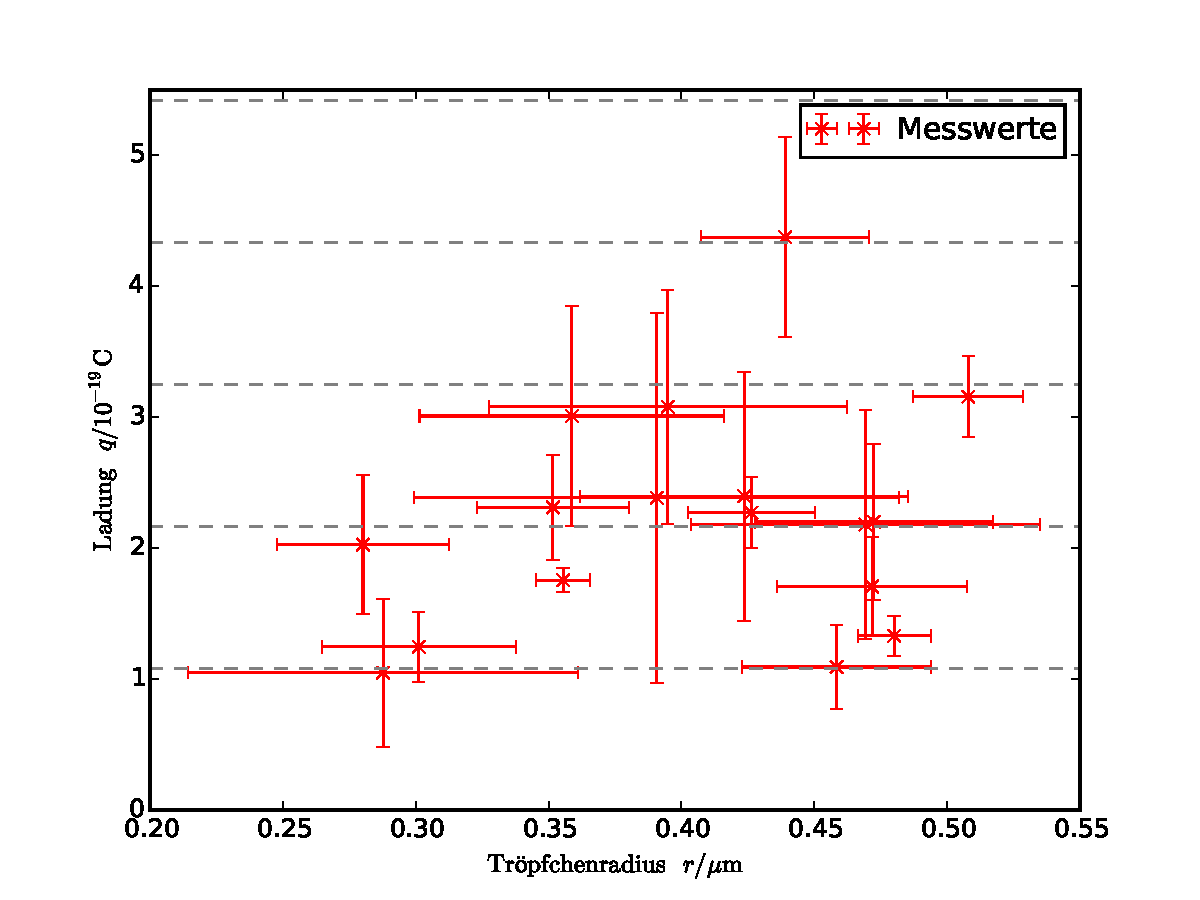
\includegraphics[width=\textwidth]{Bilder/plot_messwerte+.pdf}
	\caption{Abhängigkeit von Ladung $q$ und Radius $r$ der Tröpfchen mit eingezeichneten Vielfachen der berechneten Elementarladung.}
	\label{fig:label1}
\end{figure}
